% =========================================================
% CSC311 Final Project Report Template
% Single column, 12pt, 8 pages max.
% =========================================================

\documentclass[12pt]{article}

% ---------- Packages ----------
\usepackage[margin=1in]{geometry}
\usepackage{parskip}         % blank line between paragraphs, no indent
\usepackage{graphicx}
\usepackage{booktabs}
\usepackage{amsmath, amssymb}
\usepackage{siunitx}
\usepackage[hidelinks]{hyperref}
\usepackage{caption}
\usepackage{enumitem}
\usepackage{xcolor}
\usepackage{mathpazo}

%--------- Headers and footers ------
\usepackage{fancyhdr}
\pagestyle{fancy}
\setlength{\headheight}{14.49998pt}
\fancyhf{}
\fancyhead[L]{CSC311 Project Report}
\fancyhead[R]{Victor Jiang, Yuelin Wu, William Penn}
\fancyfoot[C]{\thepage}

% ---------- Captions & Lists ----------
\captionsetup{font=small, labelfont=bf}
\setlist[itemize]{noitemsep, topsep=2pt}
\setlist[enumerate]{noitemsep, topsep=2pt}

% ---------- Helpful macros ----------
\newcommand{\bestmodel}{\textit{[Best Model Name]}}
\newcommand{\projacc}{\textbf{[XX.XX\%]}}

% ---------- Safe figure helper ----------
\makeatletter
\newcommand{\maybeincludegraphics}[3]{%
  \begin{figure}[h]
    \centering
    \IfFileExists{#1}{%
      \includegraphics[width=0.7\linewidth]{#1}%
    }{%
      \fbox{%
        \parbox[c][0.28\textheight][c]{0.7\linewidth}{%
          \centering
          \vspace{0.5em}
          \textit{[Placeholder for \texttt{#1}]}\\
          Add your figure here.
          \vspace{0.5em}
        }%
      }%
    }%
    \caption{#2}
    \label{#3}
  \end{figure}%
}
\makeatother

% =========================================================
% Title Page
% =========================================================
\begin{document}

\begin{titlepage}
    \centering
    \vspace*{3cm}

    {\Large {CSC311: Introduction to Machine Learning} \par}
    \vspace{1cm}
    
    {\Large {Project Report} \par}
    \vspace{5cm}
    
    {\large Submitted by \par}
    
%    \vspace{0.5cm}
%    {\large Group Number}
    
    \vspace{0.5cm}
    {\large Victor Jiang, Yuelin Wu, William Penn \par}
    
    \vfill
    {\large University of Toronto \\ Winter 2026 \par}
\end{titlepage}
\clearpage
\setcounter{page}{1}

\section{Data Exploration}

\begin{figure}[h]
	\centering
	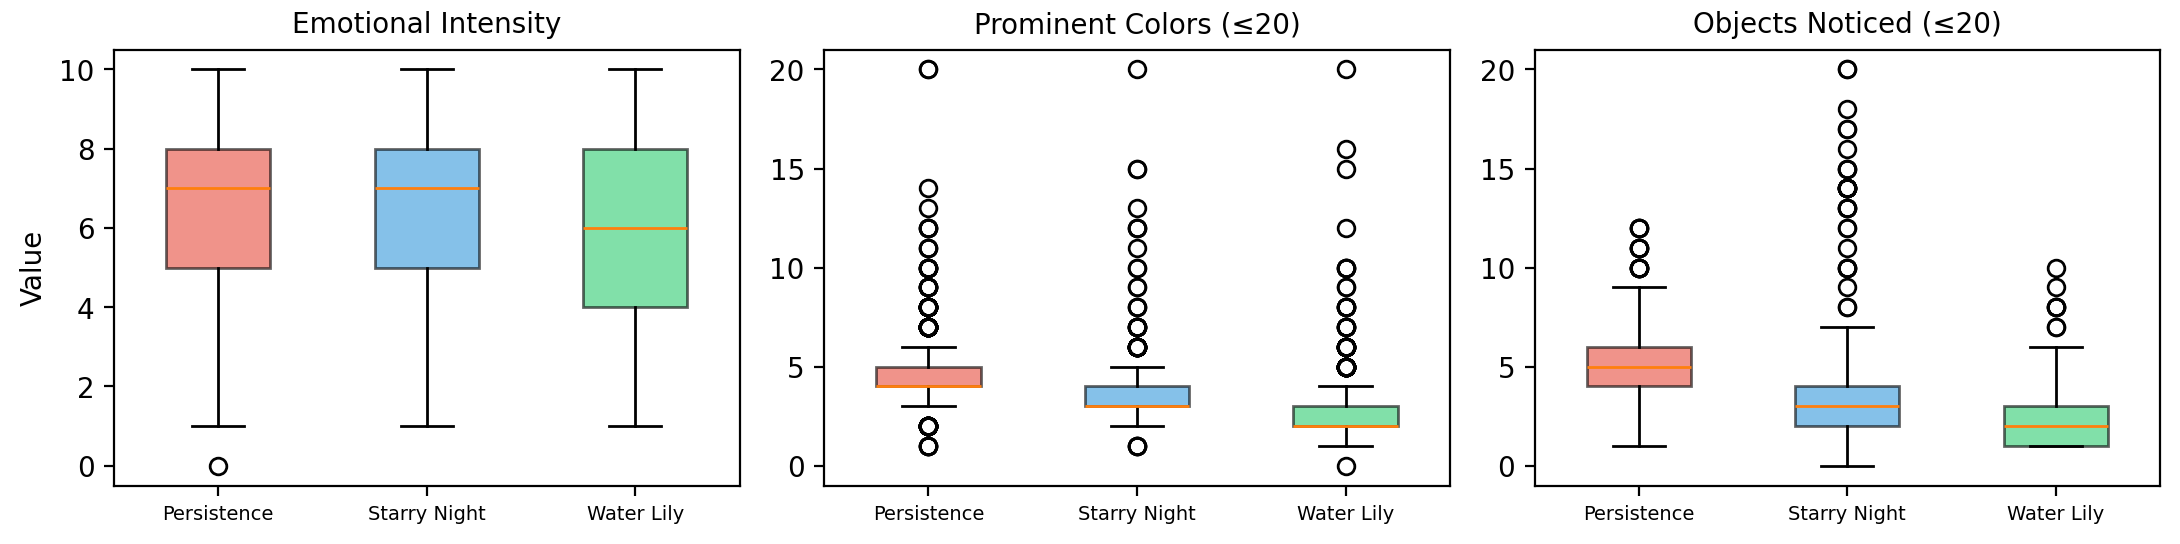
\includegraphics[width=0.9\linewidth]{numeric_boxplots.png}
	\captionsetup{width=0.9\linewidth}
	\caption{Boxplots of various numeric features by target painting, after removal of single outlier that answered 100 for both "prominent amount of colours" and "objects noticed"}
\end{figure}

First, we interpreted "On a scale of 1-10, how intense is the emotion conveyed by the artwork?" as a numeric feature, as the intensity is in a range of 1-10, and number being close indicates a similar level of intensity. Looking at \textit{Figure 1}, the distribution of emotional intensity was relatively similar across all three paintings, with the mean for "Water Lily" of around 6 being lower than the mean emotional intensity for "Persistence" and "Starry Night", both around 7. Our interpretation of this is that a lower emotional intensity may be slightly more correlated with "Water Lily" than the other two paintings.

Both "How many prominent colours do you notice in this painting?" and "How many objects caught your eye in the painting?" are counts that are best represented as numeric features. The boxplots show that "Persistence" has a slightly higher mean for both features than "Starry Night", which also has a slightly higher mean than "Water Lily". This suggests that a higher count of prominent colours and objects noticed may be slightly more likely correlated with "Persistence" and "Starry Night" than "Water Lily."

\begin{figure}[h]
	\centering
	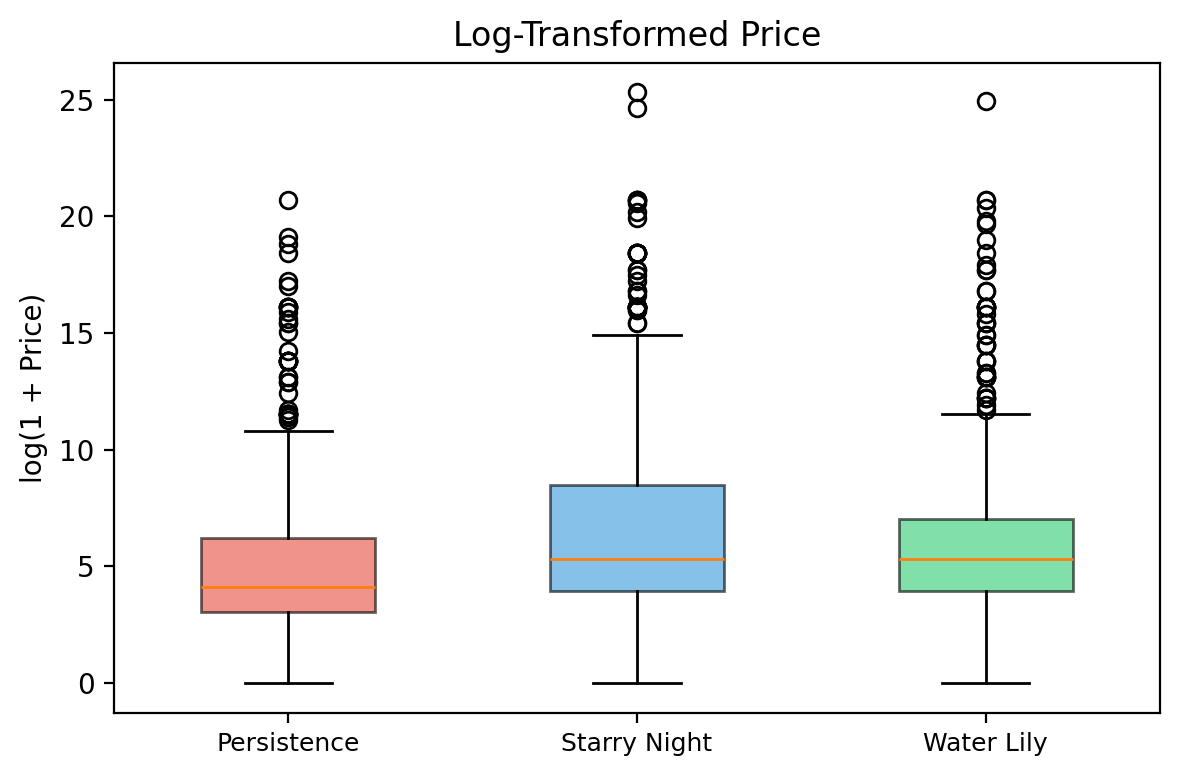
\includegraphics[width=0.4\linewidth]{log_price.png}
	\captionsetup{width=0.7\linewidth}
	\caption{Boxplots of log-transformed price by target painting, after removal of two outliers that answer $10^{60}$ and $10^{80}$}
\end{figure}

We interpreted "How much (in Canadian dollars) would you be willing to pay for this painting?" as a numeric feature as well, as the price is a continuous value. However, we log-transformed the price by $\log_{10}$ as many prices are incredibly high, making it difficult to meaningfully interpret. From \textit{Figure 2}, we can see that the distribution is relatively similar across all three paintings. Thus, we determined that the log-price may not be a very useful feature, but we included it regardless.

\begin{figure}[h]
	\centering
	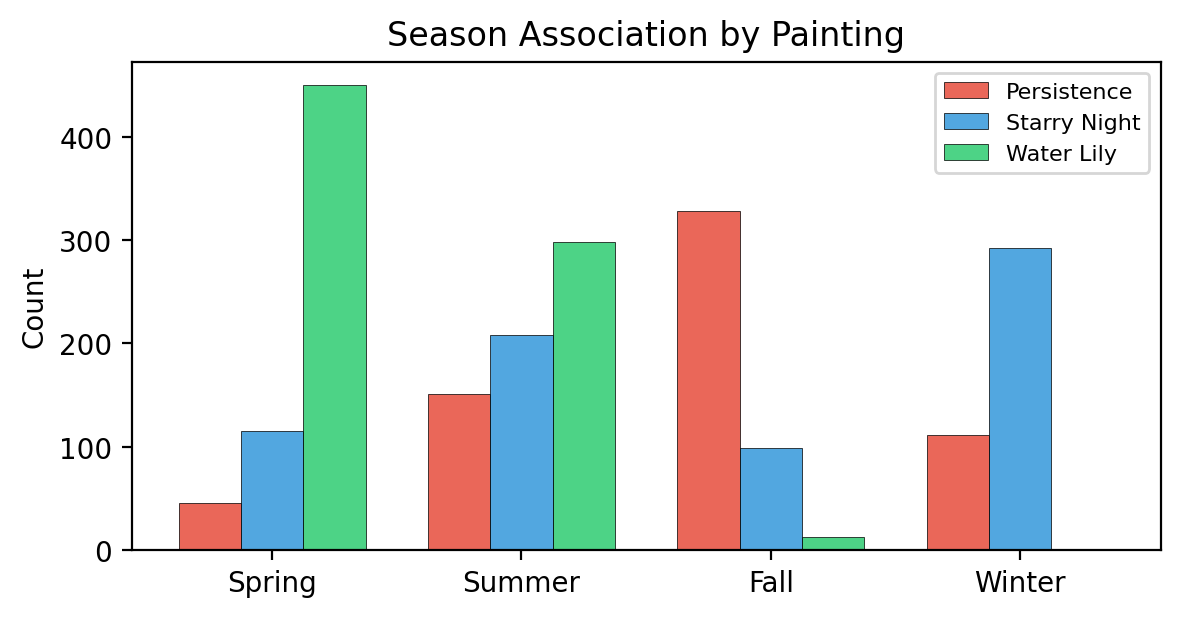
\includegraphics[width=0.5\linewidth]{season_by_class.png}
	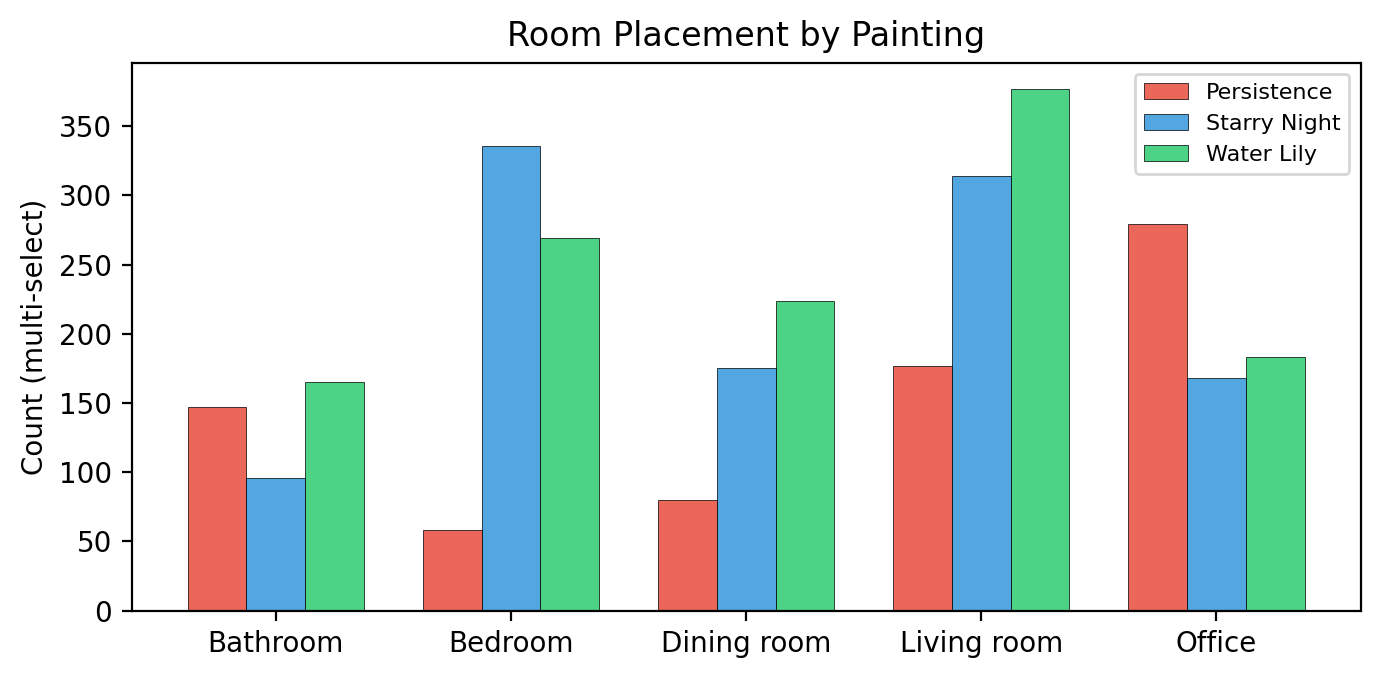
\includegraphics[width=0.49\linewidth]{room_histogram.png}
	\captionsetup{width=0.9\linewidth}
	\caption{Histogram of "Season" and "Room Placement" by target painting}
\end{figure}

We decided that "What season does this art piece remind you of?" should be treated as a categorical feature that are encoded as one-hot vectors, as all answers are one of the four seasons. From \textit{Figure 3}, we can clearly see that Spring is highly correlated with "Water Lily", Fall is highly correlated with "Persistence", and Winter is highly correlated with "Starry Night"; Summer is more so correlated with "Water Lily" than the others, but not as strongly. From this, we expect that this feature will be very useful for our model. We decided that "If you could purchase this painting, which room would you put that painting in?" is also obviously a categorical feature that should be encoded as one-hot vectors. Although it is more difficult to interpret the histogram, there are clearly correlations between various room placements and the three paintings. The "If you could view this art in person, who would you want to view it with?" feature is extremely similar and was encoded as one-hot vectors as well.

\begin{figure}[h]
	\centering
	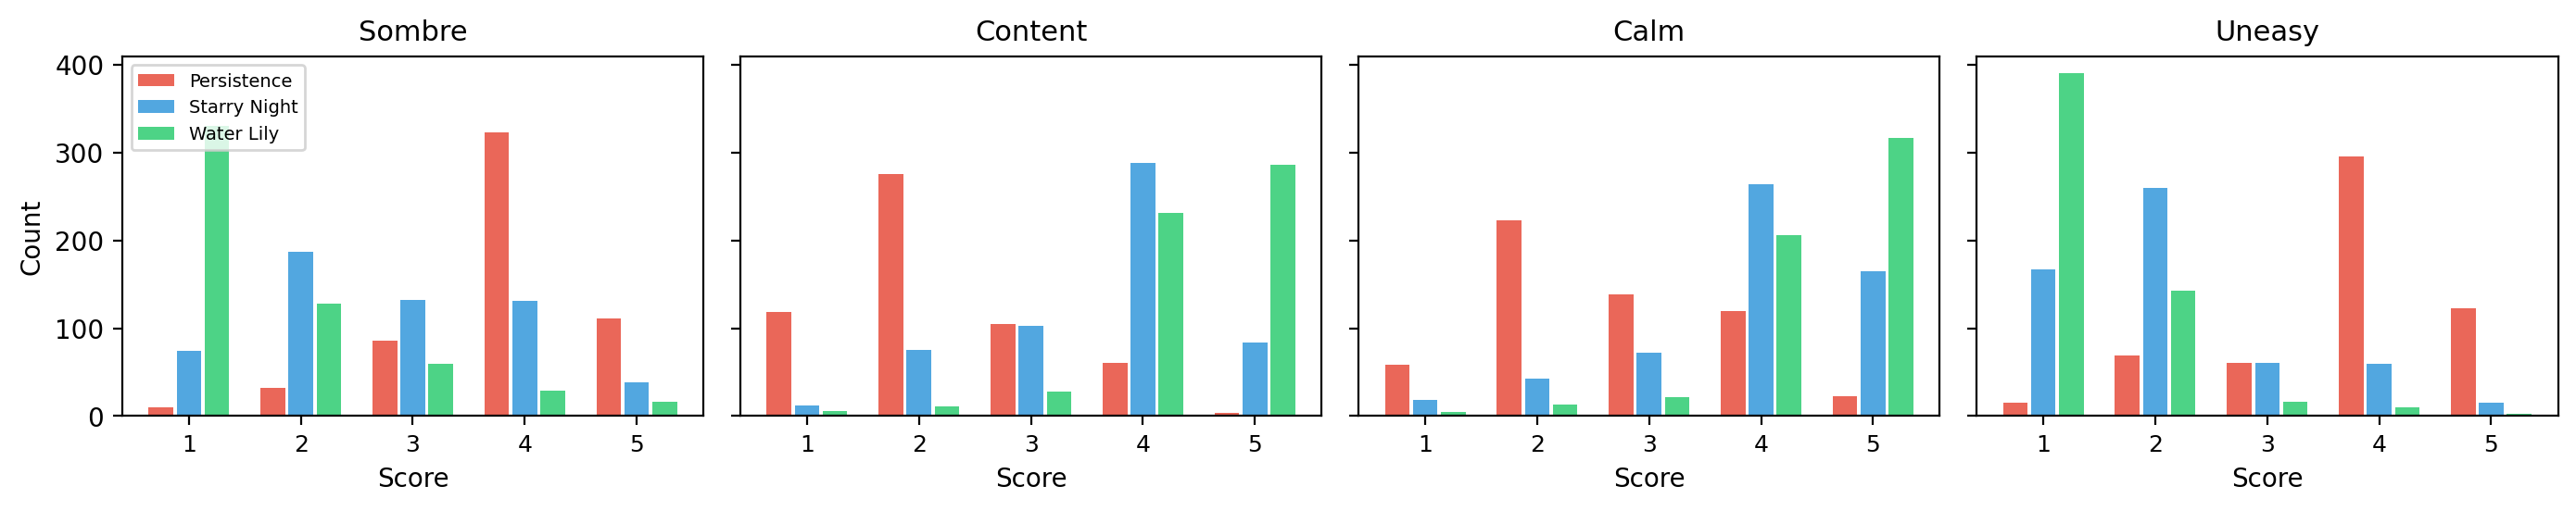
\includegraphics[width=1\linewidth]{likert_distributions.png}
	\captionsetup{width=0.7\linewidth}
	\caption{Histogram of the four likert features by target painting}
\end{figure}

We interpreted the four likert questions as essentially numeric features, as the answers are on a scale of 1-5 and the number being close indicates a similar level of feeling. There are some clear correlations present, such high "content" and "calm" feelings being more correlated with "Water Lily".

Lastly, we decided to use a Bag of Words representation for the three free response questions (description, food, soundtrack) as they are all open-ended questions with a variety of answers. We ended up not including the soundtrack feature as through ablation where we excluded the soundtrack feature from our model, we found that removing the soundtrack feature actually improved our model performance, suggesting that the soundtrack feature may be noisy and not very useful for our model.

We chose to split our data into 80\% training set and 20\% validation set, stratified so that each subset maintains the same proportion of samples from each class of target paintings. Considering the limited amount of data we are working with and the fact that a lot of the data is incomplete, instead of using a separate test set and diminishing the size of our training/validation sets, we decided to use cross-validation to evaluate our model performance.

\section{Model Exploration}

We looked at a variety of models that seemed most likely to give the best results: logistic regression, random forest classifiers, naive bayes, and MLPs. For logistic regression, we standardized the numeric features as we are performing regularization, and then we tuned the (inverse) regularization strength hyperparameter $C$. For random forest classifiers, the data input was fine the way it was, and we tuned both the number of estimators (trees in the forest) as well as the maximum depth of the trees.

We also explored using a naive bayes model. Since our data is both numeric and categorical, we explored using a Gaussian naive bayes model, which also required standardization of the numeric features. As well, we explored using a Complement naive bayes model, which was recommended by \texttt{sklearn} for imbalanced datasets and for text classification, which could be helpful for parsing the BoW features. Lastly, we explored using a MLP model, which also required standardization of the numeric features. We tuned both the hidden layer sizes and the regularization strength $\alpha$.

\section{Model Choice and Hyperparameters}

To give each model family the best chance of performing well, we evaluated our models by looking at the combination of hyperparameters that gave the model within each model family the highest validation accuracy. For example, our hyperparameter tuning for the random forest model with 200 trees can be seen below in \textit{Figure 5}, and our hyperparameter tuning for the logistic regression model can be seen below in \textit{Figure 6}. We then compared the best models from each family by evaluating their stratified 5-fold cross-validation accuracy, which acted effectively as our test set and remained consistent across all models.

\begin{figure}[h]
	\centering
	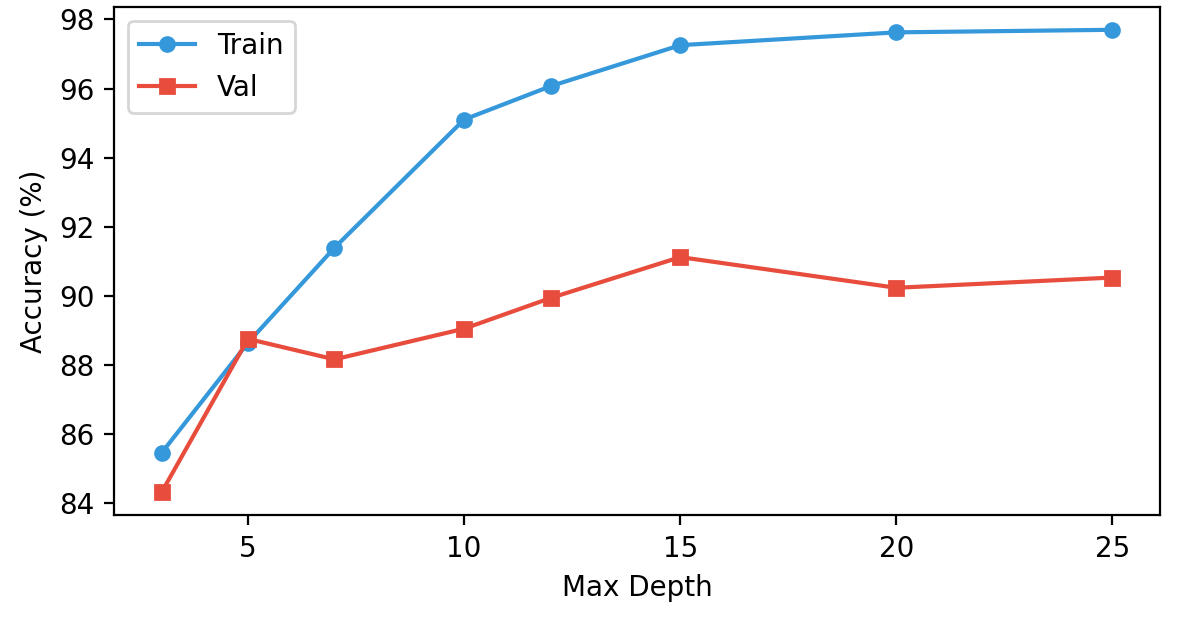
\includegraphics[width=0.6\linewidth]{rf_depth_sweep.png}
	\captionsetup{width=0.8\linewidth}
	\caption{Accuracy of random forest with 200 trees for various depths}
\end{figure}

We found that the models with the best cross-validation accuracy were a MLP with one hidden layer of 64 and $\alpha=0.01$ that had an accuracy of $0.8766\pm 0.0111$, a random forest classifier with 200 trees and a depth of 10 that had an accuracy of $0.8772\pm 0.0116$, and finally a logistic regression model with $C=0.1$ that had an accuracy of $0.8796\pm 0.0090$. As the logistic regression model had the highest cross-validation accuracy and was also the simplest model to implement, we chose the logistic regression model as our final model.

\pagebreak

For the logistic regression model, the only hyperparameter that required tuning was the inverse regularization strength $C$. We started with a large range of values for $C$ from $0.01$ to $10.0$ as seen in \textit{Figure 6}, and then narrowed down our search to values between $0.01$ and $0.2$. We found that either $C=0.05$ or $C=0.1$ would give us the best validation accuracy of 0.8935; we ultimately chose $C=0.1$ as it also had the highest training accuracy, as well as being the highest cross-validation accuracy.

\begin{figure}[h]
	\centering
	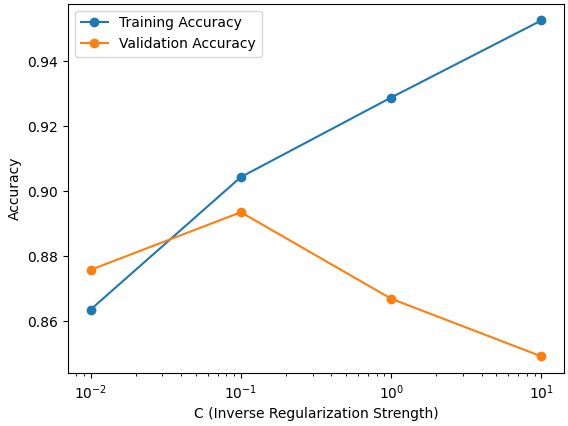
\includegraphics[width=0.5\linewidth]{log_reg_hyperpara_1.png}
	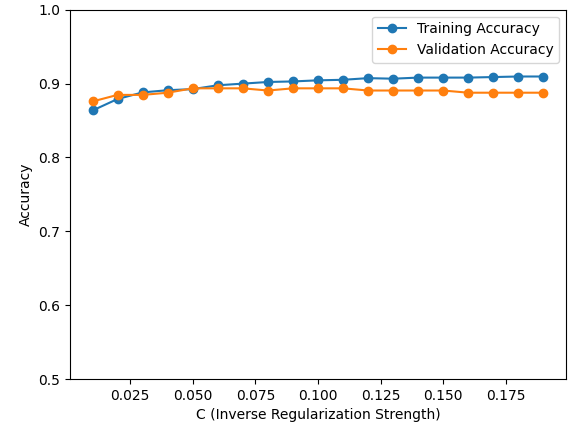
\includegraphics[width=0.49\linewidth]{log_reg_hyperpara_2.png}
	\captionsetup{width=0.7\linewidth}
	\caption{Accuracy of logistic regression for various $C$}
\end{figure}

Therefore, our final model choice for this challenge is a Logistic Regression model with an inverse regularization strength of $C=0.1$. After selecting this model, we considered what other hyperparameters we could tune, as well as any other optimizations we could make to improve model performance. First, 


First, we performed an ablation study to see whether the removal of any features would actually improve our model performance and found that the removal of the soundtrack BoW 

\section{Prediction}

\textbf{Worth 1 points. No more than 1 page.} How well would you expect your model to perform on the
test set? We are looking for:
\begin{itemize}
	\item A point estimate for your performance, \textbf{not a range}.
	\item A reasoned explanation of your expected model performance, with empirical
	evidence supporting your explanation. 
	You are not graded on the closeness of your estimate to the final test accuracy,
	but you are graded on your reasoning.
\end{itemize}


\section{Workload Distribution}

Describe what each person in the group contributed
to the project. A 1-2 sentence description of each person's role is sufficient.
Each student's description must be written by that student in order for them
to receive credit for the project.


\section{References}

Use references whenever appropriate (e.g., when you consult textbooks, research papers, online tutorials, or external code). Cite in the text using \verb|\cite{}|. For example, let's cite the two references provided in the \texttt{.bib} file \cite{bishop2006prml,hastie2009esl}. (Replace these with your own references.)

\bibliographystyle{plain}
\bibliography{references}

\end{document}
